\documentclass[12pt, titlepage]{article}

\usepackage{fullpage}
\usepackage[round]{natbib}
\usepackage{multirow}
\usepackage{booktabs}
\usepackage{tabularx}
\usepackage{graphicx}
\usepackage{float}
\usepackage{hyperref}
\usepackage[shortlabels]{enumitem}
\usepackage{amsmath, mathtools}
\usepackage{amsfonts}
\usepackage{amssymb}
\usepackage{colortbl}
\usepackage{xr}
\usepackage{longtable}
\usepackage{xfrac}
\usepackage{siunitx}
\usepackage{caption}
\usepackage{pdflscape}
\usepackage{afterpage}
\usepackage{titlesec}
\usepackage{array}
%\usepackage{showframe}
\hypersetup{
    colorlinks,
    citecolor=blue,
    filecolor=black,
    linkcolor=red,
    urlcolor=blue
}
\usepackage{graphicx}
\graphicspath{ {./images/} }
\usepackage{caption}
\usepackage{enumitem}
\usepackage{xcolor}
\usepackage{listings}
\usepackage{geometry}
\usepackage{amsfonts}

\input{../Comments}
%% Common Parts

\newcommand{\progname}{Chess Connect} % PUT YOUR PROGRAM NAME HERE
\newcommand{\authname}{Team \#4,
\\ Alexander Van Kralingen
\\ Arshdeep Aujla
\\ Jonathan Cels
\\ Joshua Chapman
\\ Rupinder Nagra} % AUTHOR NAMES without MacIDs 

\usepackage{hyperref}
    \hypersetup{colorlinks=true, linkcolor=blue, citecolor=blue, filecolor=blue,
                urlcolor=blue, unicode=false}
    \urlstyle{same}

\newcommand{\projectoverview}{

The Chess Connect project allows two users to play a game of chess on a physical board with the information being transmitted to an online web application over Bluetooth.
Currently, there is no way for players to seamlessly switch between playing on a physical board and playing online, but Chess Connect intends to change this by creating a central platform that will provide flexibility and remove barriers for new players looking to learn the game.

}

% https://tex.stackexchange.com/a/409782
\colorlet{mygray}{black!30}
\colorlet{mygreen}{green!60!blue}
\colorlet{mymauve}{red!60!blue}

\lstset{
  backgroundcolor=\color{gray!10}, 
  basicstyle=\small,
  columns=fullflexible,
  breakatwhitespace=false,
  breaklines=true,
  captionpos=b,
  commentstyle=\color{mygreen},
  extendedchars=true,
  frame=single,
  keepspaces=true,
  keywordstyle=\color{blue}, 
  language=c++, 
  numbers=none,
  numbersep=5pt,
  numberstyle=\tiny\color{blue},
  rulecolor=\color{mygray}, 
  showspaces=false,
  showtabs=false,
  stepnumber=5,
  stringstyle=\color{mymauve}, 
  tabsize=3,
  title=\lstname 
}

\newcounter{acnum}
\newcommand{\actheacnum}{AC\theacnum}
\newcommand{\acref}[1]{AC\ref{#1}}

\begin{document}

\title{System Verification and Validation Report for \progname{}} 
\author{\authname}
\date{\today}
	
\maketitle

\pagenumbering{roman}

\section{Revision History}

\begin{tabularx}{\textwidth}{p{3cm}p{2cm}X}
\toprule {\bf Date} & {\bf Version} & {\bf Notes}\\
\midrule
2023-03-04 & Arshdeep Aujla & Added Template for Nonfunctional Requirements\\
2023-03-05 & Arshdeep Aujla & Added Table for functional requirements, traceability matrix\\
2023-03-07 & Jonathan Cels & Added functional requirement test reports\\
2023-03-08 & Joshua Chapman & Added changes due to testing, Trace to Modules\\
2023-03-08 & Alexander Van Kralingen & Added Arduino unit tests example\\
2023-03-08 & Jonathan Cels & Added nonfunctional requirement test reports\\
2023-03-08 & Arshdeep Aujla & Added reflection appendix\\
2023-03-08 & Alexander Van Kralingen & Completed Code Coverage Metrics section\\
\bottomrule
\end{tabularx}

~\newpage

\section{Symbols, Abbreviations and Acronyms}

\renewcommand{\arraystretch}{1.2}
\begin{tabular}{l l} 
    \toprule		
    \textbf{symbol} & \textbf{description}\\
    \midrule 
    T & Test\\
  FSM & Finite State Machine\\
    TBD & To Be Determined\\
    LCD & Liquid Crystal Display\\
    LED & Light Emitting Diode\\
    Engine Move & Good chess move, calculated by a chess engine\\
    Legal Move & Chess move that is allowed according to the rules\\
    Illegal Move & Chess move that is not allowed according to the rules\\
    ADC & Analog to Digital Converter\\
  \bottomrule
\end{tabular}\\

Refer to SRS Section 1 for an extensive list of used symbols, abbreviations, and acronyms.

\newpage

\tableofcontents

\listoftables %if appropriate

\listoffigures %if appropriate

\newpage

\pagenumbering{arabic}

\section{Functional Requirements Evaluation}
Refer to the VnV Plan for descriptions of the tests derived to evaluate the functional requirements.
\subsection{Game Active State}

\begin{table}[H]
    \centering
        \setlength{\leftmargini}{0cm}
        \begin{tabular}{| >{\centering\arraybackslash}m{1cm} | 
            >{\centering\arraybackslash}m{2.5cm} | 
            >{\centering\arraybackslash}m{4cm} | 
            >{\centering\arraybackslash}m{3cm} |
            >{\centering\arraybackslash}m{3cm} |
            >{\centering\arraybackslash}m{1.5cm} |}
        \hline
        \rowcolor[gray]{0.9}
        Test & Input & Expected & Actual & Notes & Result\\
        \hline
        GA-1 & Draw/resign button pressed while game active. & System variable `gameInProgress' set to false. &  System variable configured correctly. &  & Pass \\
        \hline
        GA-2 & Start game button pressed while game active. & System variable `gameInProgress' remains true. &  System variable configured correctly. &  & Pass \\
        \hline
        GA-3 & User mode button pressed while game active. & System variable `currMode' changed to represent the selected user mode. &  User mode unchanged. & Design changed, user mode not switchable while a game is active. & Rework \\
        \hline
        GA-4 & Start game button pressed while game inactive. & System variable `gameInProgress' set to true, `currFEN' variable is set to the starting FEN. &  System variables configured correctly. &  & Pass \\
        \hline
        GA-5 & Move made that results in stalemate or checkmate according to the rules of chess while game inactive. & System variable `gameInProgress' set to false. &  System variable configured correctly. &  & Pass \\ 
        \hline
        \end{tabular}
    \caption{Active State Functional Requirements Results}
\end{table}

\subsection{Game Inactive State}

\begin{table}[H]
    \centering
        \setlength{\leftmargini}{0cm}
        \begin{tabular}{| >{\centering\arraybackslash}m{1cm} | 
            >{\centering\arraybackslash}m{2.5cm} | 
            >{\centering\arraybackslash}m{4cm} | 
            >{\centering\arraybackslash}m{3cm} |
            >{\centering\arraybackslash}m{3cm} |
            >{\centering\arraybackslash}m{1.5cm} |}
        \hline
        \rowcolor[gray]{0.9}
        Test & Input & Expected & Actual & Notes & Result\\
        \hline
        GI-1 & Start game button pressed while game inactive. & System variable `gameInProgress' set to true. & System variable configured correctly. &  & Pass \\
        \hline
        GI-2 & User mode button pressed while game inactive. & User mode unchanged. & System variable configured correctly. & Design changed, user mode is now switchable (only) while a game is inactive. & Rework \\
        \hline
        GI-3 & Draw/resign button pressed while game inactive. & System variable `gameInProgress' remains false. & System variable configured correctly. &  & Pass \\
        \hline
        GI-4 & Piece moved while game inactive. & System variable `currFEN' is unchanged. & System variable configured correctly. &  & Pass \\
        \hline
        GI-5 & Draw/resign button pressed, or move made that results in stalemate or checkmate according to the rules of chess while game active. & Game termination and winner are displayed on LCD screen. & Display updates correctly. &  & Pass \\
        \hline
        \end{tabular}
    \caption{Inactive State Functional Requirements Results}
\end{table}

\subsection{Normal Mode}

\begin{table}[H]
    \centering
        \setlength{\leftmargini}{0cm}
        \begin{tabular}{| >{\centering\arraybackslash}m{1cm} | 
            >{\centering\arraybackslash}m{2.5cm} | 
            >{\centering\arraybackslash}m{4cm} | 
            >{\centering\arraybackslash}m{3cm} |
            >{\centering\arraybackslash}m{3cm} |
            >{\centering\arraybackslash}m{1.5cm} |}
        \hline
        \rowcolor[gray]{0.9}
        Test & Input & Expected & Actual & Notes & Result\\
        \hline
        NB-1 & Piece moved while in normal mode. & Game state is updated to reflect piece movement. & Game state updated correctly. &  & Pass \\
        \hline
        NB-2 & Resign button pressed while in normal mode. & System variable `gameInProgress' set to false. & System variable configured correctly. &  & Pass \\
        \hline
        NB-3 & Draw button pressed while in normal mode. & System variable `gameInProgress' set to false. & System variable configured correctly. &  & Pass \\
        \hline
        ND-1 & Game state updated while in normal mode. & Updated game state is transmitted to the web application via Bluetooth. & Game state transmitted correctly. &  & Pass \\
        \hline
        NA-1 & Web application receives updated game state while in normal mode. & Update to game state is reflected on web application display. & Display updates correctly. &  & Pass \\
        \hline
        NA-2 & Game termination occurs while in normal mode. & Game termination and winner are displayed on web application display. & Display updates correctly. &  & Pass \\
        \hline
        \end{tabular}
    \caption{Normal Mode Functional Requirements Results}
\end{table}

\pagebreak
\subsection{Engine Mode}
    \begin{longtable}{| >{\centering\arraybackslash}m{1cm} | 
        >{\centering\arraybackslash}m{2.5cm} | 
        >{\centering\arraybackslash}m{4cm} | 
        >{\centering\arraybackslash}m{3cm} |
        >{\centering\arraybackslash}m{3cm} |
        >{\centering\arraybackslash}m{1.5cm} |}
    \hline
    \rowcolor[gray]{0.9}
    Test & Input & Expected & Actual & Notes & Result\\
    \hline
    EB-1 & Piece moved while in engine mode. & Game state is updated to reflect piece movement. & Game state updated correctly. &  & Pass \\
    \hline
    EB-2 & Resign button pressed while in engine mode. & System variable `gameInProgress' set to false. & System variable configured correctly. &  & Pass \\
    \hline
    EB-3 & Draw button pressed while in engine mode. & System variable `gameInProgress' set to false. & System variable configured correctly. &  & Pass \\
    \hline
    EB-4 & Engine moves transmitted from the web application to microcontroller. & Engine moves are displayed on the LCD screen. & Display updated correctly. &  & Pass \\
    \hline
    ED-1 & Game state updated while in engine mode. & Updated game state is transmitted to the web application via Bluetooth. & Game state transmitted correctly. &  & Pass \\
    \hline
    ED-2 & Engine moves are calculated by the web application. & Calculated engine moves are transmitted from the web application to the microcontroller via Bluetooth & Moves transmitted correctly. & Only one engine move currently calculated, more planned in future revisions. & Partial Pass \\
    \hline
    \pagebreak 
    \hline
    \rowcolor[gray]{0.9}
    Test & Input & Expected & Actual & Notes & Result\\
    \hline
    EA-1 & Web application receives updated game state while in engine mode. & Update to game state is reflected on web application display. & Display updates correctly. &  & Pass \\
    \hline
    EA-2 & Engine moves are calculated by the web application. & Calculated engine moves are displayed on web application display. & Engine moves are not displayed. & Not implemented, planned in future revisions. & TBD \\
    \hline
    EA-3 & Game termination occurs while in engine mode. & Game termination and winner are displayed on web application display. & Display updates correctly. &  & Pass \\
    \hline
    \caption{Engine Mode Functional Requirements Results}\\
\end{longtable}

\pagebreak

\subsection{Beginner Mode}
    \begin{longtable}{| >{\centering\arraybackslash}m{1cm} | 
        >{\centering\arraybackslash}m{2.5cm} | 
        >{\centering\arraybackslash}m{4cm} | 
        >{\centering\arraybackslash}m{3cm} |
        >{\centering\arraybackslash}m{3cm} |
        >{\centering\arraybackslash}m{1.5cm} |}
    \hline
    \rowcolor[gray]{0.9}
    Test & Input & Expected & Actual & Notes & Result\\
    \hline
    BB-1 & Piece moved while in beginner mode. & Game state is updated to reflect piece movement. & Game state updated correctly. &  & Pass \\
    \hline
    BB-2 & Piece picked up and held while in beginner mode. & LEDs on board indicate legal moves. & Correct LEDs light up. &  & Pass \\
    \hline
    BB-3 & Piece moved such that an illegal move is made while in beginner mode. & LEDs on board indicate illegal move. & Correct LEDs light up. & Not implemented, planned in future revisions. & TBD \\
    \hline
    BB-4 & Resign button is pressed while in beginner mode. & System variable `gameInProgress' set to false. & System variable configured correctly. &  & Pass \\
    \hline
    BB-5 & Draw button is pressed while in beginner mode. & System variable `gameInProgress' set to false. & System variable configured correctly. &  & Pass \\
    \hline
    BD-1 & Game state is updated while in beginner mode. & Updated game state is transmitted to the web application via Bluetooth. & Game state transmitted correctly. &  & Pass \\
    \hline
    \pagebreak 
    \hline
    \rowcolor[gray]{0.9}
    Test & Input & Expected & Actual & Notes & Result\\
    \hline
    BA-1 & User selects chess instructions in web application. & Web application displays detailed rules for how to play chess. & N/A & Not implemented, planned in future revisions. & TBD \\
    \hline
    BA-2 & Web application receives updated game state while in beginner mode. & Update to game state is reflected on web application display. & Display updates correctly. &  & Pass \\
    \hline
    \caption{Beginner Mode Functional Requirements Results}\\
\end{longtable}
    
\pagebreak

\section{Nonfunctional Requirements Evaluation}

Many of the nonfunctional requirements outlined in the VnV plan are left for revision 1, as much of the external testing relies on the product being more completed and accessible to a wider audience.
Some external user testing was done, specifically for NFT-4 and NFT-5, and is detailed in the Performance section.

\subsection{Look and Feel}

Look and feel testing will be performed for revision 1, as though it is functional, this part of the product is not ready for external user testing.
		
\subsection{Usability and Humanity}

Usability testing will be performed for revision 1, as though it is functional, this part of the product is not ready for external user testing.

\subsection{Performance}

\begin{table}[H]
    \centering
        \setlength{\leftmargini}{0cm}
        \begin{tabular}{| >{\centering\arraybackslash}m{2cm} | 
            >{\centering\arraybackslash}m{2.5cm} | 
            >{\centering\arraybackslash}m{3cm} | 
            >{\centering\arraybackslash}m{2cm} |
            >{\centering\arraybackslash}m{4cm} |
            >{\centering\arraybackslash}m{1.5cm} |}
        \hline
        \rowcolor[gray]{0.9}
        Test & Input & Expected & Actual & Notes & Result\\
        \hline
        NFT-4 & Experiment performed as detailed below. & Average LED response time over all trials is less than 0.5 seconds. & Average response time was 0.488 seconds. & This value is close to the 0.5 second limit, and may be subject to human error. Further testing will be done with more trials for revision 1 to ensure this requirement is met. & Pass \\
        \hline
        NFT-5 & Experiment performed as detailed below. & Maximum single response time of any trial is less than 1 second. & Maximum response time was 0.72 seconds. &  & Pass \\
        \hline
        NFT-6 & N/A & N/A & N/A & Not tested, as the system is currently subject to a 2-second delay before refreshing. Will be tested for revision 1. & TBD \\
        \hline
        NFT-7 & N/A & N/A & N/A & Not tested, as the system is currently subject to a 2-second delay before refreshing. Will be tested for revision 1. & TBD \\
        \hline
        \end{tabular}
    \caption{Performance Non-Functional Requirements Results}
\end{table}

\newpage
The following table holds data for NFT-4 and NFT-5. Three external users, all familiar with the rules of chess, were each asked to perform the following experiment in beginner mode 5 times:
\medskip
\\
Pick up an arbitrary piece and suspend it in the air. Wait until the board visually indicates the possible moves for the suspended piece. The time between the user picking up 
the piece and the board's LED indicators turning on was measured and recorded.

\begin{table}[H]
    \centering
    \setlength{\leftmargini}{0cm}
    \begin{tabular}{| >{\centering\arraybackslash}m{4cm} | 
        >{\centering\arraybackslash}m{3cm} |
        >{\centering\arraybackslash}m{3cm} | 
        >{\centering\arraybackslash}m{3cm} |}
    \hline
    \rowcolor[gray]{0.9}
    & User 1 & User 2 & User 3 \\
    \hline
    Trial 1 & 0.49s & 0.48s & 0.36s \\
    \hline
    Trial 2 & 0.65s & 0.69s & 0.27s \\
    \hline
    Trial 3 & 0.53s & 0.33s & 0.52s \\
    \hline
    Trial 4 & 0.72s & 0.34s & 0.49s \\
    \hline
    Trial 5 & 0.42s & 0.51s & 0.52s \\
    \hline
    Total Average & \multicolumn{3}{c|}{\textbf{0.488s}}\\
    \hline
    \end{tabular}
\caption{Experimental Results of Performance Testing}
\end{table}

The following scatter plot shows the experimental results visually. The average, shown in green, falls just below the 
required 0.5 second threshold, and all points are well below the maximum acceptable response time of 1 second.

\begin{figure}[H]
    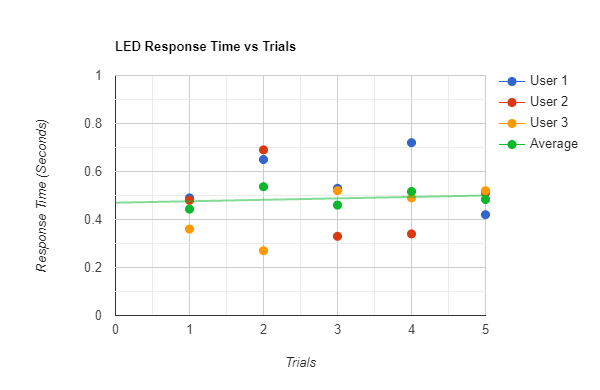
\includegraphics[scale=0.93]{performanceScatterPlot}
    \caption{Experimental Results of Performance Testing}
\end{figure}

\newpage
\subsection{Health and Safety}

\begin{table}[H]
\centering
    \setlength{\leftmargini}{0cm}
    \begin{tabular}{| >{\centering\arraybackslash}m{1cm} | 
        >{\centering\arraybackslash}m{4cm} | 
        >{\centering\arraybackslash}m{3cm} | 
        >{\centering\arraybackslash}m{3cm} |
        >{\centering\arraybackslash}m{2.5cm} |
        >{\centering\arraybackslash}m{1.5cm} |}
    \hline
    \rowcolor[gray]{0.9}
    Test & Input & Expected & Actual & Notes & Result\\
    \hline
    NFT-8 & 10 sample wires were chosen while the product was running. Their current and voltage were measured, and power was calculated using those measurements. & All power measurements below safe limits. & All power measurements below safe limits. & Measurements far below any safety thresholds. & Pass \\
    \hline
    \end{tabular}
\caption{Health and Safety Non-Functional Requirements Results}
\end{table}

The following table holds data for NFT-8. 

\begin{table}[H]
    \centering
    \setlength{\leftmargini}{0cm}
    \begin{tabular}{| >{\centering\arraybackslash}m{1cm} | 
        >{\centering\arraybackslash}m{3cm} |
        >{\centering\arraybackslash}m{1.5cm} | 
        >{\centering\arraybackslash}m{2cm} |
        >{\centering\arraybackslash}m{2cm} |
        >{\centering\arraybackslash}m{2.5cm} |
        >{\centering\arraybackslash}m{2.5cm} |}
    \hline
    \rowcolor[gray]{0.9}
    Wire \# & Wire Description & Gauge & Current (Amps) & Voltage (Volts) & Calculated Power (Watts) & Maximum power (Watts) \\
    \hline
    1 & Hall sensor 1 with black piece & 20 & 0.04 & 1.6 & 0.064 & 7.5 \\
    \hline
    2 & Hall sensor 32 with no piece & 20 & 0.03 & 1 & 0.03 & 7.5 \\
    \hline
    3 & Hall sensor 64 with white piece & 20 & 0.02 & 0.6 & 0.012 & 7.5 \\
    \hline
    4 & Arduino power line & 10 & 0.5 & 5 & 2.5 & 75 \\
    \hline
    5 & ADC 1 & 20 & 0.01 & 5 & 0.05 & 7.5 \\
    \hline
    6 & ADC 4 & 20 & 0.02 & 5 & 0.1 & 7.5 \\
    \hline
    7 & ADC clock & 20 & 0.05 & 5 & 0.25 & 7.5 \\
    \hline
    8 & Wall power supply (L) & 8 & 0.75 & 110 & 47.631 & 120 \\
    \hline
    9 & Wall power supply (G) & 8 & 0.01 & 0 & 0 & 120 \\
    \hline
    10 & Bluetooth RX & 20 & 0.02 & 5 & 0.1 & 7.5 \\
    \hline
    \end{tabular}
\caption{Experimental Results of Health and Safety Testing}
\end{table}

\subsection{Precision and Accuracy}

Precision and accuracy testing will be performed for revision 1, as though it is functional, this part of the product is not ready for external user testing.

\subsection{Capacity}

\begin{table}[H]
\centering
    \setlength{\leftmargini}{0cm}
    \begin{tabular}{| >{\centering\arraybackslash}m{1cm} | 
        >{\centering\arraybackslash}m{2.5cm} | 
        >{\centering\arraybackslash}m{4cm} | 
        >{\centering\arraybackslash}m{3cm} |
        >{\centering\arraybackslash}m{3cm} |
        >{\centering\arraybackslash}m{1.5cm} |}
    \hline
    \rowcolor[gray]{0.9}
    Test & Input & Expected & Actual & Notes & Result\\
    \hline
    NFT-10 & A relatively complex chess FEN position was transmitted via Bluetooth to the web application while in engine mode. & The measured memory usage of the web application is less than 1GB. & The maximum measured memory value was 1187.4 MB, as measured by Windows task manager. & Memory usage will increase in future revisions, as more engine moves will be calculated at a higher depth. & Pass \\
    \hline
    \end{tabular}
\caption{Capacity Non-Functional Requirements Results}
\end{table}

\subsection{Security}

\begin{table}[H]
\centering
    \setlength{\leftmargini}{0cm}
    \begin{tabular}{| >{\centering\arraybackslash}m{1cm} | 
        >{\centering\arraybackslash}m{2.5cm} | 
        >{\centering\arraybackslash}m{4cm} | 
        >{\centering\arraybackslash}m{3cm} |
        >{\centering\arraybackslash}m{3cm} |
        >{\centering\arraybackslash}m{1.5cm} |}
    \hline
    \rowcolor[gray]{0.9}
    Test & Input & Expected & Actual & Notes & Result\\
    \hline
    NFT-11 & Bluetooth connection to web application severed. & Web application alert that the connection has been lost. & N/A & Not implemented, planned in future revisions. & TBD \\
    \hline
    NFT-12 & Power connection to system is severed, and then restored after a short time frame. & The game state data is stored in local memory and is unchanged after power is restored. & Game state data is properly stored. &  & Pass \\
    \hline
    \end{tabular}
\caption{Security Non-Functional Requirements Results}
\end{table}

\section{Unit Testing} \label{UnitTest}

  Unit testing is a crucial aspect of software development that involves testing individual units or components of a software application in isolation from the rest of the system. It provides us with a way to ensure that each unit of code is functioning as intended and that it integrates seamlessly with other parts of the software application. By identifying defects and bugs early in the development cycle, unit testing helps reduce the overall time spent on software development while also improving the quality and reliability of the final product. Additionally, unit tests serve as a form of documentation, helping us understand how different components of the system are supposed to interact and ensuring that future modifications do not break existing functionality. We implemented unit testing to ensure our project was robust, maintainable, and of high quality. As mentioned in the VnV Plan, the React Testing Library was used for the Javascript unit tests. Additionally, with the inclusion of many hardware related components in our project, most of our testing is done manually, leaving very few tests that require being automated. 
  \\\\
  Creating unit tests for the Embedded software required several of Arduino's built in functionality to be simulated. This included serial communication functions,
  pin setup (input or output), reading from and writing to pins, and time delays. Additionally, binary values neded to be setup to simulate a sequence of events 
  such as values recorded from a hall sensor, or LEDs turning on or off. All of this is handled in the 
  \href{../../test/EmbeddedTest/ArduinoTest/MockArduinoController.cpp}{MockArduinoController.cpp} file, which holds the SerialStream and PinSimulation classes,
  as well as several functions for interacting with the hardware.

  Rather than unit testing every function in normal operation, individual functions were tested to ensure correct outputs from simulated inputs. Integration 
  with the system was completed physically with the Arduino exectuing the program. An example of the test for hardware reading is given below. 
  \newpage 
\begin{lstlisting}
    void testReadPiece()
    {
        setupBoard(); 
        
        // Simulate picking a piece 
        organizedHallValues[0][1] = randHall(NO_COLOUR);  
        mapHallValuesToSensors(); 
        PinSim.reWritePin(hallRx[0]); 
        writeAdcRow(hallRx[0], rawHallValues[0]); 

        // NO_PIECE, NO_COLOUR 
        Square expectedSquare = Square(0,1);    

        // Checkpick() function inside Arduino's loop should catch this,
        // updating the pieces on the board 
        loopArduino();  

        // Make sure the state changes to PIECE_LIFTED ('l')
        check(assert_equal('l', gameState), __FUNCTION__, __LINE__);  

        // Make sure the square in the board array is updated successfully
        check(assert_equal(expectedSquare, currentBoard[0][1]), __FUNCTION__, __LINE__);  
    }
\end{lstlisting}

  The rest of the tests follow a similar format of setting up the initial state, simulating an input and comparing the expected output. Several similar tests were 
  performed with different piece types, positions and piece colours to cover edge cases. Only one test of each type in a group testing the same function with 
  different inputs and outputs has been included in the table below. Test inputs and outputs are provided in natural language due to the size of the initial values 
  (8$\times$8 struct representing the board state, 64 blocks of 12 digit binary numbers representing the hall sensor values, one change in piece).

\newgeometry{left=0.5cm}
  \begin{longtable}{| p{.33\textwidth} | p{.21\textwidth} | p{.21\textwidth} | p{.21\textwidth} | p{.07\textwidth} |}
    \hline
    \rowcolor[gray]{0.9}
    Test & Input & Expected & Actual & Result\\
    \hline
    testReadPiece & random Hall sensor value between 140 and 310 (no piece reading) corresponding to square B1 & Square B1 resets piece value to NO\_PIECE & currentBoard[0][1] holds NO\_PIECE, NO\_COLOUR  & pass \\
    \hline
    testHighlightPawnValidMoves & Pawn lifted from starting position (A2) & A3, A4 light up & A3, A4 pins read output HIGH & pass \\
    \hline
    testHighlightKnightValidMoves & Knight lifted from starting position (B1)& A3, C3 light up & pins read output HIGH & pass \\
    \hline
    testHighlightBishopValidMoves & Bishop lifted from C1 after D2 Pawn to D3, and G7 Pawn to G5 & C2, E3, F4, G5 light up & C2, E3, F4, G5 pins read output HIGH & pass \\
    \hline
    testHighlightRookValidMoves & Rook lifted from D4 (no other pieces moved) & light up A4, B4, C4, D4, E4, F4, G4, H4, D3, D5, D6, D7 & A4, B4, C4, D4, E4, F4, G4, H4, D3, D5, D6, D7 pins read output HIGH & pass \\
    \hline
    testHighlightQueenValidMoves & Queen lifted from D4 (no other pieces moved) & light up C3, C4, C5, B6, A7, D5, D6, D7, E5, F6, G7, E3, E4 & C3, C4, C5, B6, A7, D5, D6, D7, E5, F6, G7, E3, E4 pins read output HIGH & pass \\
    \hline
    testHighlightKingValidMoves & King lifted (E1) with castling available & light up E2, F1, G1 & E2, F1, G1 pins read output HIGH & pass \\
    \hline
    testPieceToChar & Piece(QUEEN, BLACK) & 'q' & 'q' & pass \\
    \hline
    testValidateFENString & Piece sequence from start: 1. e4 e5 2. Nf3 Nc6 3. d4 & {\scriptsize rnbqkbnr/pppp1ppp/ 4p3/8/4P3/5N2/ PPPP1PPP/RNBQKB1R w KQkq - 1 4} & {\scriptsize rnbqkbnr/pppp1ppp/ 4p3/8/4P3/5N2/ PPPP1PPP/RNBQKB1R w KQkq - 1 4} & pass \\
    \hline
    testGameStartValid & black piece on row 1 while all other pieces are white & false & false & pass \\
    \hline
    inStalemate & rnbqkbnr/\-pppppppp\-/8/8/8/8/\-PPPPPPPP/\-RNBQKBNR w KQkq - 0 1 & false & false & pass \\
    \hline 
    inCheckmate & rnb1kbnr/\-pppp1ppp\-/8/4p3\-/5PPq/8/\-PPPPP2P/\-RNBQKBNR \-w KQkq - 1 3 & true & true & pass \\
    \hline
    \caption{Unit Test functions}
  \end{longtable}

\restoregeometry

\section{Changes Due to Testing}
The results detailed in the above tests prompted a number of design changes in 
the hardware, embedded and web application systems. Outlined below are the 
changes made as result. 

\subsection{Embedded Testing} 
Testing the finite state machine located in the electrical system resulted in 
incorrect functionality according to the design. A finite state machine was 
designed to control the functionality of the electrical system dictated by the
user. It allows users to change modes and have control over the performance 
of the board. The initial implementation of the FSM utilized a slow clock speed
and certain inputs were missed as a result. The new solution is to increase the
clock speed of the FSM and include buffers within the states to increase the
robustness of the system. 
\newline
\newline
Easy mode provides the functionality of possible moves for pieces on the board.
When a piece is lifted, the available squares are highlighted. During testing of 
the function, there were a number of edge cases that were not covered such as 
castling, en passant and check scenarios. The proposed solution was to increase
the robustness of the algorithm and maintain logs of the game to account for
these edge cases. 

\subsection{Hardware Testing}
Testing the hall sensor piece detection circuits at scale uncovered issues
with sensitivity of the sensors. At scales of four or more sensors in series, 
the sensitivity of the reading was too large. Initial solutions included 
improvement of the hardware. This included improvement of the power supply, 
grounding and sensors themselves. These solutions did not solve the issue. As 
a result, the requirements of the sensors have been changed to sense north and 
south poles exclusively. The functionality of individual piece detection was not
feasible. 
\newline
\newline
Assembly of the revision one chess board displayed issues with robustness of the
connections between mechanical and electrical assemblies. Temporary connection 
was established with electrical and duct tape. The electrical system suspended 
below the mechanical system. After testing of the board, connection points began 
to fail and separation occured. The solution for revision two is assembly of the
mechanical and electrical systems simultaneously. The two systems are assembled 
together and the robustness of the system is increased.

\subsection{Web Application Testing}
Integration of the web application with the embedded system revealed an error 
with the implementation of polling in the web application. Polling required 
handling of constant data transmission between systems. Issues were clear with 
required data and processing dedicated to this communicatin. One of the proposed
solutions is the implementation of a refresh to erase the stored data. This 
eliminates the data size issue. A second solution is the introduction of sockets
which eliminates polling entirely and solves the data size and processing issues. 


\begin{itemize}
  \item Initially, the game was only allowed to start while white and black were on specific sides. Code changed to support either side as starting position.
\end{itemize}
  

\section{Automated Testing}
\subsection{C++}
  Since Arduino files are .ino and cannot be build using a g++ compiler, a build script has been created to convert the file to a .cpp filetype, compile it with
  g++, execute it and watch the result. The error code is the number of errors which used by GitHub Actions to determine the success of all of the unit tests. Errors
  are written to a log file and recorded for future reference. Unit tests are run in this method to verify changes to the code. Tests must all pass before merging
  into main. Please refer to \hyperref[UnitTest]{Unit Testing} for details on the tests ran in build script.

\subsection{React Testing Library}
The React Testing Library was used for testing our React components. 
Its function was to assist writing tests that simulate user 
interactions with their application, allowing us to ensure that the components 
are working as intended. The library provides a set of utilities that make it 
easy to test React components by interacting with them as a user would, rather 
than relying on implementation details. This means that tests written with this library
are more resilient to changes in the underlying codebase, and 
provide better coverage of the user experience. Overall, the React Testing Library
was an important tool to ensure the quality and reliability
of our frontend application.
		
\section{Trace to Requirements \& Modules}

\begin{longtable}{| p{.20\textwidth} | p{.4\textwidth} | p{.4\textwidth}|}
  \hline
  Test & Requirement & Module\\
  \hline
  GA-1 & GA1 & M2\\
  \hline
  GA-2 & GA2 & M2\\
  \hline
  GA-3 & GA3 & M2\\
  \hline
  GA-4 & GA6 & M2\\
  \hline
  GA-5 & GA7 & M2, M5, M11\\
  \hline
  GI-1 & GI1 & M2\\
  \hline
  GI-2 & GI2 & M2, M11\\
  \hline
  GI-3 & GI3 & M2\\
  \hline
  GI-4 & GI4 & M2, M4\\
  \hline
  GI-5 & GI5, GI6 & M2, M5, M11\\
  \hline
  NB-1 & NB1 & M2, M11\\
  \hline
  NB-2 & NB2 & M2, M11\\
  \hline
  NB-3 & NB3 & M2, M11\\
  \hline
  ND-1 & ND1 & M2, M11\\
  \hline
  NA-1 & NA1, NA2 & M2, M6, M8, M11\\
  \hline
  NA-2 & NA3 & M2, M5, M11\\
  \hline
  EB-1 & EB1 & M2, M5, M11\\
  \hline
  EB-2 & EB2 & M2, M11\\
  \hline
  EB-3 & EB3 & M2, M11\\
  \hline
  EB-4 & EB4 & M10, M14\\
  \hline
  ED-1 & ED1 & M5, M6, M8, M12\\
  \hline
  ED-2 & ED2 & M14\\
  \hline
  EA-1 & EA1, EA2 & M5, M6, M8, M11\\
  \hline
  EA-2 & EA3, EA4, EA5 & M14\\
  \hline
  EA-3 & EA6 & M5, M6, M8, M9\\
  \hline
  BB-1 & BB1 & M4, M5, M11\\
  \hline
  BB-2 & BB2 & M4, M5, M11\\
  \hline
  BB-3 & BB3 & M4, M5, M11\\
  \hline
  BB-4 & BB4 & M2, M5, M11\\
  \hline
  BB-5 & BB5 & M2, M5, M11\\
  \hline
  BD-1 & BD1 &  M2, M5, M11\\
  \hline
  BA-1 & BA1 & M10, M11\\
  \hline
  BA-2 & BA2 & M2, M8, M9\\
  \hline
  NFT1 & LF3 &\\
  \hline
  NFT2 & UH5 &\\
  \hline
  NFT3 & UH6 &\\
  \hline
  NFT4 & PR1 &\\
  \hline
  NFT5 & PR2 &\\
  \hline
  NFT6 & PR3 &\\
  \hline
  NFT7 & PR4 &\\
  \hline
  NFT8 & PR6 &\\
  \hline
  NFT9 & PR7 &\\
  \hline
  NFT10 & PR10 &\\
  \hline
  NFT11 & SR4 &\\
  \hline
  NFT12 & SR3 &\\
  \hline
\caption{Requirements Traceability Matrix}
\end{longtable}
		
\section{Trace to Modules}		

\section{Code Coverage Metrics}

The code coverage was measured through a combination of Function coverage and Path coverage. Since the number of possible moves in a chess game is an 
atronomically large number, complete path coverage would be close to 0\%. Therefore, only paths that produced a change in state (game start, switch to beginner
mode, draw game, etc.), significant change in values (piece taken, piece lifted, piece placed, etc.), or a standard operation of the game (following piece movement
from the board to the web app) were considered as code paths.

Arduino executes the following 2 functions during runtime:

\begin{center}
  setup() $\rightarrow$ loop()
\end{center}

All code paths occur in the loop() function. After pins are initialized and communication modules are connected, an example of the path through the
code taken by one of actions is as follows:

\begin{center}
  gameCommand=BEGINNER\_MODE $\rightarrow$ readHallSensors() $\rightarrow$ identifyColors() $\rightarrow$ resetChessBoard() 
  $\rightarrow$ gameState=PLAY\_GAME $\rightarrow$ updateBoard() $\rightarrow$ readHallSensors() $\rightarrow$ etc\dots
\end{center}

\begin{table}[H]
  \centering
  \setlength{\leftmargini}{0cm}
      \begin{tabular}{| >{\centering\arraybackslash}m{2cm} | 
          >{\centering\arraybackslash}m{3cm} |
          >{\centering\arraybackslash}m{2cm} |
          >{\centering\arraybackslash}m{2cm} |
          >{\centering\arraybackslash}m{3cm} |}
      \hline
      \rowcolor[gray]{0.9}
      Coverage & Number of Functions/Paths & Number Tested & \% Covered & Notes\\
      \hline
      Function & 60 & 44 & 73\% & A list of all functions covered can be found in \hyperref[FunctionsCovered]{Appendix \ref{FunctionsCovered}} \\
      \hline
      Path & 41 & 32 & 78\% & A list of all paths considered can be found in \hyperref[CodePaths]{Appendix \ref{CodePaths}} \\
      \hline
      \end{tabular}
  \caption{Code Coverage Metrics}
  \end{table}

\pagebreak
\appendix
\section{Coverage Metrics Details}
\subsection{Functions Covered}\label{FunctionsCovered}

\begin{itemize}
  \item[\checkmark] pieceToChar
  \item[\checkmark] charToPiece
  \item[\checkmark] detectNewPiece
  \item[\checkmark] readHall
  \item[\checkmark] readHallRow
  \item[\checkmark] adjust
  \item[$\times$] printHall
  \item[\checkmark] setupHallSensors
  \item[$\times$] setupLEDs
  \item[\checkmark] readHallSensors
  \item[\checkmark] resetChessBoard
  \item[$\times$] LightAllPieces
  \item[\checkmark] LightSquare
  \item[\checkmark] movePiece
  \item[$\times$] printColors
  \item[$\times$] printBoard
  \item[\checkmark] identifyColors
  \item[$\times$] updateBoard
  \item[\checkmark] gameStartValid
  \item[$\times$] assignPieces
  \item[\checkmark] rowToFen
  \item[\checkmark] boardToFen
  \item[\checkmark] sendFen
  \item[\checkmark] checkPick
  \item[\checkmark] checkPlace
  \item[\checkmark] lightUp
  \item[\checkmark] lightValidSquare
  \item[\checkmark] flash
  \item[\checkmark] highlightPawnMoves
  \item[\checkmark] highlightKnightMoves
  \item[\checkmark] highlightBishopMoves
  \item[\checkmark] highlightRookMoves
  \item[\checkmark] highlightQueenMoves
  \item[\checkmark] highlightKingMoves
  \item[\checkmark] btComm
  \item[$\times$] appendCharToStr
  \item[\checkmark] setEngineBoxText
  \item[$\times$] makeEngineBox
  \item[$\times$] makeStartButton
  \item[$\times$] makeWhiteResignButton
  \item[$\times$] makeDrawButton
  \item[$\times$] makeBlackResignButton
  \item[$\times$] makeGameModeButtons
  \item[\checkmark] selectNormalMode
  \item[\checkmark] selectEngineMode
  \item[\checkmark] selectBeginnerMode
  \item[\checkmark] resignGame
  \item[\checkmark] drawGame
  \item[\checkmark] startGame
  \item[\checkmark] changeMode
  \item[\checkmark] updateState
  \item[\checkmark] parseWebPayload
  \item[\checkmark] getData
  \item[\checkmark] sendData
  \item[\checkmark] App
  \item[$\times$] errFunction
  \item[$\times$] storeData
  \item[\checkmark] writeArduino
  \item[$\times$] btSerial.on("found")
  \item[\checkmark] router.get('/')
  \item[\checkmark] router.post('/')
\end{itemize}

\subsection{Code Paths}\label{CodePaths}

% [$\times$]
\bf{Paths considered}
\begin{itemize}
  \item[\checkmark] board start with no pieces
  \item[\checkmark] board start with pieces in correct positions
  \item[\checkmark] board start with pieces in wrong positions
  \item[\checkmark] game start in Beginner Mode
  \item[\checkmark] game start in Normal Mode
  \item[\checkmark] game start in Engine Mode
  \item[\checkmark] move white piece in Beginner Mode
  \item[\checkmark] move white piece in Normal Mode
  \item[\checkmark] move white piece in Engine Mode
  \item[\checkmark] move black piece in Beginner Mode
  \item[\checkmark] move black piece in Normal Mode
  \item[$\times$] move black piece in Engine Mode
  \item[\checkmark] move pawn from start in Beginner Mode
  \item[\checkmark] move pawn from start in Normal Mode
  \item[\checkmark] move pawn from start in Engine Mode
  \item[\checkmark] pawn En Passant in Beginner Mode
  \item[\checkmark] pawn En Passant in Normal Mode
  \item[\checkmark] pawn En Passant in Engine Mode
  \item[\checkmark] move bishop from random square in Beginner Mode
  \item[$\times$] move bishop from random square in Normal Mode
  \item[\checkmark] move bishop from random square in Engine Mode
  \item[\checkmark] move knight from random square in Beginner Mode
  \item[$\times$] move knight from random square in Normal Mode
  \item[$\times$] move knight from random square in Engine Mode
  \item[\checkmark] move queen from random square in Beginner Mode
  \item[$\times$] move queen from random square in Normal Mode
  \item[$\times$] move queen from random square in Engine Mode
  \item[\checkmark] move king from random square in Beginner Mode
  \item[$\times$] move king from random square in Normal Mode
  \item[$\times$] move king from random square in Engine Mode
  \item[\checkmark] king castling in Beginner Mode
  \item[\checkmark] king castling in Normal Mode
  \item[\checkmark] king castling in Engine Mode
  \item[$\times$] move piece to illegal spot
  \item[\checkmark] white capture black piece
  \item[\checkmark] black capture white piece
  \item[\checkmark] white king in check
  \item[\checkmark] black king in check
  \item[\checkmark] white king in checkmate
  \item[\checkmark] black king in checkmate
  \item[\checkmark] resign button pressed
  \item[\checkmark] draw button pressed
\end{itemize}

\section{Reflection}
The majority of the tests planned out in the VnV Plan were carried out as expected and reported in the VnV Report. 
Some differences in the tests were due to a rework of the requirements, and modifying what is in scope for the first iteration of the project.\\

Two tests were not carried out as planned because the requirements changed since the creation of the VnV Plan. These tests were GA-3 and GI-2.
These tests were both related to the changing the game state. Initially, functional requirements outlined that the user should be able to change the games mode
regardless if they are currently in the active state or inactive state. On a second consideration, it was decided that the mode should only be able to be changed if
the user is in the inactive mode. Therefore the tests GA-3 and GI-1 were no long applicable and not reported in this report. \\

A few tests for functional and non-functional requirements were not completed due to the scope of the project changing. The requirements changed because 
they were decided that they weren't mandatory for a working product. It was also not feasible for these requirements to be met during the timeline of the course.
These tests that were descoped were ED-2, EA-2, BB-3, BA-1, NFT-6, NFT-7, and NFT-11.\\

In a future VnV planning, emphasis will need to be made to ensure that the requirements are solidified before the tests are created, and that all of the requirements need to
be feasible to be met during the project's timeline.

\bibliographystyle{plainnat}

\nocite{*}\bibliography{../../refs/References}

\end{document}